\documentclass[12pt]{article}

\usepackage[compact,small]{titlesec}
\usepackage[hmargin={0.6in,0.6in}, vmargin={0.5in, 0.01in}]{geometry}
\usepackage{graphicx, wrapfig, hyperref, url, denselists}
\usepackage{url, xcolor}
\newcommand{\email}[1]{\href{mailto:#1}{\normalfont\texttt{#1}}}


\usepackage{graphicx}
\usepackage{transparent}
\usepackage{eso-pic}

\AddToShipoutPicture*{
    \put(0,0){
        \parbox[b][\paperheight]{\paperwidth}{%
            \vfill
            \centering
            {\transparent{0.15}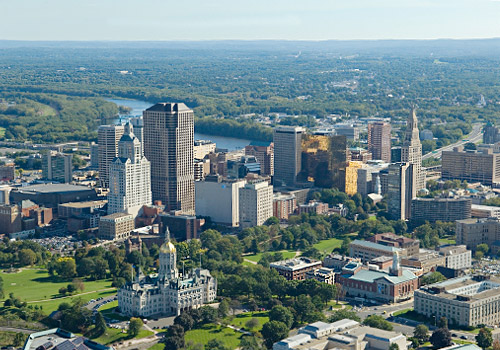
\includegraphics[height=\paperheight]{hartford}}%
            \vfill
        }
    }
}


\begin{document}

\pagestyle{empty}

\definecolor{dukeblue}{rgb}{0.0, 0.0, 0.61}

\noindent\fcolorbox{blue}{dukeblue}{%
\begin{minipage}[m]{1.8in}

\includegraphics[width=\linewidth]{NESS19}
\end{minipage}}%
\begin{minipage}[m]{5.5in}
\begin{center}
{\bf\Large  The 33rd New England Statistics Symposium\\[8pt]
 Statistical Data Science in Action}\\[8pt]
{\bf\large \url{https://symposium.nestat.org/}}\\[8pt]
{\bf\large Department of Statistics, University of Connecticut}\\[8pt]
{\bf May 15--17, 2019, Hilton Hartford, CT}
\end{center}
\end{minipage}

\bigskip
The Department of Statistics of the University of Connecticut is proud to host the first remodeled, 3-day NESS after the establishment of the New England Statistical Society, on May 15–17, 2019.

\paragraph{Four Short Courses} Wednesday, May 15, 2019
% (\url{https://symposium.nestat.org/short-courses.html})

\noindent
1. (Full-day) Intermediate Machine Learning: Key Concepts and Techniques, by Dr. David Rosenberg (Bloomberg)

\noindent
2. (Full-day) Big Data Analytics and Deep Learning, by Dr. Ming Li (Amazon) and Dr. Hui Lin (Netlify)

\noindent
3. (Half-day) Practical Visualization for Data Scientists, by Dr. Xiaoyue Cheng (University of Nebraska at Omaha)

\noindent
4. (Half-day) Introduction to Multilevel Modeling, by Dr. Min Zhu (SAS)

\paragraph{Plenary Presentations} (\url{https://symposium.nestat.org/plenary-speakers.html})

\noindent\textsf{Opening Keynote} Thursday, May 16, 2019

Dr. Sam Kou, Harvard University: Big Data, Google and Disease Detection: A Statistical Adventure

Dr. David Rosenberg / Dr. Amanda Stent, Bloomberg: Machine Learning for Structured and Unstructured Data in Finance

\noindent\textsf{Banquet Talk} Thursday, May 16, 2019

Dr. Anthony D'Amico,   Dana-Farber Cancer Institute and Brigham \& Women's Hospital: Improving Patient Outcomes in Prostate Cancer by Partnering Statistics and Medicine

\noindent\textsf{Chernoff Lecture} Friday, May 17, 2019

The inaugural Chernoff Awardee whose identity remains a secret until the closing Award Ceremony.

\paragraph{Invited Sessions}
A total of 60 sessions (10 tracks) cover a wide spectrum of areas of Statistical Data Science in Action. % with speakers from academia, industry, and government agencies. % Special panel discussions on career development and non-technical skills for statisticians and data scientists are of special interest to the next generation work force.
Proposal submission deadline is March 18, 2019

\paragraph{Contributed Poster Session} Thursday, May 16, 2019.
Contribution is welcome from everyone.
Presenting students automatically enter the student poster award competition.

\paragraph{Student Competitions} Students are encouraged to participate in three events.

\textsf{Stat-a-thon} (\url{http://statathon.stat.uconn.edu/})
A statistical data science invention marathon sponsored by Travelers. Two data challenges have been released: Connecticut Housing; and Customer Retention. Students form teams to compete. The deadline of submission is April 26, 2019.

\textsf{IBM Student Paper Competition} Submission deadline is April 1, 2019.

\textsf{Student Poster Competition} Submission deadline is April 26, 2019.


\paragraph{Registration}
All participants in the conference must register. The registration fee
covers conference materials, breakfasts, lunches and tea
breaks. Members of the New England Statistical Society
(\url{https://nestat.org}) receive discounts in pricing. To register,
please complete the on-line registration form at
\url{https://symposium.nestat.org/registration.php}.


\paragraph{Venue}
Hilton Hartford will offer discount rate to the conference
participants until April 18th or until the group block is sold out. To
book, please visit
\url{https://symposium.nestat.org/venue.html}.


\vfill

\begin{center}
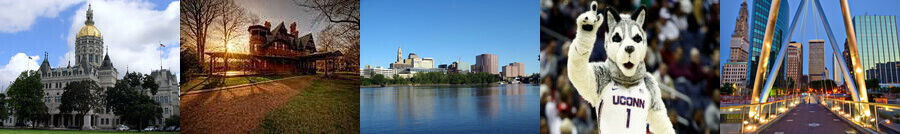
\includegraphics[width=\textwidth]{hartford-banner}
\end{center}

\end{document}
